\section{Vel composition}
\label{sec:Vel composition}
\begin{theorem}
  Given a node $x$ and a nonempty set $Y$ such that $E(x,Y)$, then for all nodes $a,b$ such that $V(a,x)$ and either $V(a,y)$ or $V(b,y)$ for all $y \in Y$ we have that either $V(a,a)$ or $V(a,b)$.
\end{theorem}
This general property will later be proven directly, but we will start by giving an exhaustive proof of the base case where $Y=\{ y \}$.
This will give us a good intuition of how the general proof will look like.
\subsection{Proving the base case}
\label{sub:Proving the base case}
In the base case we have a node $x$ such that $E(x,\{ y \})$ and nodes $a$ and $b$ such that $V(a,x)$ and either $V(a,y)$ or $V(b,y)$.
We will show that these conditions implies either $V(a,a)$ or $V(a,b)$.

The figure below illustrates our two possible situations, where a solid arrow represents an edge while dashed lines represents vels:
\[
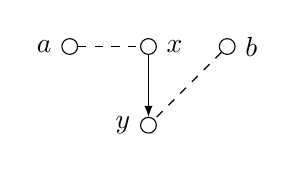
\begin{tikzpicture}
  [point/.style={circle,draw,inner sep=0pt,minimum size=2mm}]
  \node (a) at (0,1) [point,label=left:$a$] {};
  \node (b) at (2,1) [point,label=right:$b$] {};

  \node (x) at (1,1) [point,label=right:$x$] {};
  \node (y) at (1,0) [point,label=left:$y$] {};

  \draw [-latex] (x) to (y);
  \draw [dashed] (a) to (x);
  \draw [dashed] (b) to (y);
\end{tikzpicture}
\quad\quad\quad
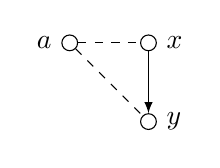
\begin{tikzpicture}
  [point/.style={circle,draw,inner sep=0pt,minimum size=2mm}]
  \node (a) at (0,1) [point,label=left:$a$] {};

  \node (x) at (1,1) [point,label=right:$x$] {};
  \node (y) at (1,0) [point,label=right:$y$] {};

  \draw [-latex] (x) to (y);
  \draw [dashed] (a) to (x);
  \draw [dashed] (a) to (y);
\end{tikzpicture}
\]
At this point, we have two cases to cover:
The one where there is a vel between $a$ and $y$, and the case with a vel between $b$ and $y$.
The following proof will cover the second case, but it turns out that the first case will have a perfectly equivalent proof.
We will come back to this later, and we will actively use this fact in the general proof.

Now that we have established our assumption, $V(a,x),V(b,y),E(x,\{y\})$, we will use our earlier definition of a vel to expand the assumption into four cases:
\begin{enumerate}[(i)]
  \item $\poo(a,c), \poe(x,c), \poo(b,d), \poe(y,d), E(x,\{y\})$
  \item $\poo(a,c), \poe(x,c), \poe(b,d), \poo(y,d), E(x,\{y\})$
  \item $\poe(a,c), \poo(x,c), \poo(b,d), \poe(y,d), E(x,\{y\})$
  \item $\poe(a,c), \poo(x,c), \poe(b,d), \poo(y,d), E(x,\{y\})$
\end{enumerate}
The figure bellow illustrates how these paths are arranged:
\[
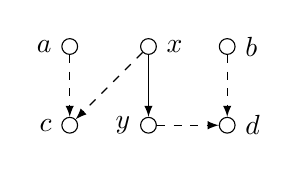
\begin{tikzpicture}
  [point/.style={circle,draw,inner sep=0pt,minimum size=2mm}]
  \node (a) at (0,1) [point,label=left:$a$] {};
  \node (b) at (2,1) [point,label=right:$b$] {};

  \node (x) at (1,1) [point,label=right:$x$] {};
  \node (y) at (1,0) [point,label=left:$y$] {};

  \node (c) at (0,0) [point,label=left:$c$] {};
  \node (d) at (2,0) [point,label=right:$d$] {};

  \draw [-latex] (x) to (y);
  \draw [-latex,dashed,label=left:$o$] (a) to (c);
  \draw [-latex,dashed,label=left:$e$] (x) to (c);
  \draw [-latex,dashed,label=right:$o$] (b) to (d);
  \draw [-latex,dashed,label=above:$e$] (y) to (d);
\end{tikzpicture}
\]
\clearpage
\subsection{2OR Proof (i)}
\label{sub:2OR Proof (i)}
\begin{prooftree*}[downwards]
  \Hypo{V_o(a,b)}
  \Infer1[def]{\ax{\poo(b,d)},\poe(a,d)}
  \Infer1[C1]{\ax{\poo(a,c)},\peo(c,d)}
  \Infer1[C2]{\ax{\poe(y,d)},P^f_o(c,y)}
  \Infer1[L3]{E(c,\{y\})}
  \Infer1[(=)]{\ax{E(x,\{y\})}, x=c}
  \Hypo{V_o(a,b)}
  \Infer1[def]{\ax{\poo(b,d)},\poe(a,d)}
  \Infer1[C1]{\ax{\poo(a,c)},\peo(c,d)}
  \Hypo{V_o(a,b)}
  \Infer1[def]{\ax{\poo(a,c)},\poe(b,c)}
  \Infer1[C1]{\ax{\poo(b,d)},\peo(d,c)}
  \Infer2[B2]{\peo(y,c),\ax{\poe(y,d)}}
  \Infer2[S3]{\ax{\poe(x,c)},\ax{E(x,\{y\})}}
\end{prooftree*}
\subsection{2OR Proof (ii)}
\label{sub:2OR Proof (ii)}
\begin{prooftree*}[downwards]
  \Hypo{V_o(a,b)}
  \Infer1[def]{\ax{\poe(b,d)},\poo(a,d)}
  \Infer1[C1]{\ax{\poo(a,c)},\pee(c,d)}
  \Infer1[C2]{\ax{\poo(y,d)},P^f_o(c,y)}
  \Infer1[L3]{E(c,\{y\})}
  \Infer1[(=)]{\ax{E(x,\{y\})}, x=c}
  \Hypo{V_o(a,b)}
  \Infer1[def]{\ax{\poe(b,d)},\poo(a,d)}
  \Infer1[C1]{\ax{\poo(a,c)},\pee(c,d)}
  \Hypo{V_o(a,b)}
  \Infer1[def]{\ax{\poo(a,c)},\poe(b,c)}
  \Infer1[C3]{\ax{\poe(b,d)}\poe(d,c)}
  \Infer2[B1]{\peo(y,c),\ax{\poo(y,d)}}
  \Infer2[S3]{\ax{\poe(x,c)},\ax{E(x,\{y\})}}
\end{prooftree*}
\subsection{2OR Proof (iii)}
\label{sub:2OR Proof (iii)}
\begin{prooftree*}[downwards]
  \Hypo{V_o(a,b)}
  \Infer1[def]{\ax{\poo(b,d)},\poe(a,d)}
  \Infer1[C3]{\ax{\poe(a,c)},\poe(c,d)}
  \Hypo{V_o(a,b)}
  \Infer1[def]{\ax{\poe(a,c)},\poo(b,c)}
  \Infer1[C1]{\ax{\poo(b,d)},\pee(d,c)}
  \Infer2[B4]{\pee(y,c),\ax{\poe(y,d)}}
  \Infer1[S1]{\ax{\poo(x,c)},\ax{E(x,\{ y \})}}
\end{prooftree*}
\subsection{2OR Proof (iv)}
\label{sub:2OR Proof (iv)}
\begin{prooftree*}[downwards]
  \Hypo{V_o(a,b)}
  \Infer1[def]{\ax{\poe(b,d)},\poo(a,d)}
  \Infer1[C3]{\ax{\poe(a,c)},\poo(c,d)}
  \Hypo{V_o(a,b)}
  \Infer1[def]{\ax{\poe(a,c)},\poo(b,c)}
  \Infer1[C3]{\ax{\poe(b,d)},\poo(d,c)}
  \Infer2[B3]{\pee(y,c),\ax{\poo(y,d)}}
  \Infer1[S1]{\ax{\poo(x,c)},\ax{E(x,\{ y \})}}
\end{prooftree*}
